\documentclass[10pt]{beamer}
\usepackage[utf8]{inputenc}
\usepackage{graphicx}
\usepackage{mathtools}
\usetheme{CambridgeUS}
\usecolortheme{dolphin}

% Set up hyperref once and configure colors
\usepackage{hyperref}
\hypersetup{
    colorlinks=true,
    linkcolor=blue,
    linktocpage
}

% Custom colors
\definecolor{myNewColorA}{RGB}{118,193,188}
\definecolor{myNewColorB}{RGB}{106,172,150}
\definecolor{myNewColorC}{RGB}{94,150,218}
\setbeamercolor*{palette primary}{bg=myNewColorC}
\setbeamercolor*{palette secondary}{bg=myNewColorB, fg=white}
\setbeamercolor*{palette tertiary}{bg=myNewColorA, fg=white}
\setbeamercolor*{titlelike}{fg=myNewColorA}
\setbeamercolor*{title}{bg=myNewColorA, fg=white}
\setbeamercolor*{item}{fg=myNewColorA}
\setbeamercolor*{caption name}{fg=myNewColorA}
\usefonttheme{professionalfonts}

\titlegraphic{
\includegraphics[height=1.5cm]{../CommonFigures/Universidad_Panamericana-logo.jpg}}

\setbeamerfont{title}{size=\large}
\setbeamerfont{subtitle}{size=\small}
\setbeamerfont{author}{size=\small}
\setbeamerfont{date}{size=\small}
\setbeamerfont{institute}{size=\small}
\title[Universidad Panamericana]{}
\subtitle{FreeRTOS Architecture Part 1}
\author[]{Name}
\institute[ltonix@up.edu.mx]{Universidad Panamericana}
\date[Presentation \today]{Presentation \today}

\AtBeginSection[]{
  \begin{frame}
  \vfill
  \centering
  \begin{beamercolorbox}[sep=8pt,center,shadow=true,rounded=true]{title}
    \usebeamerfont{title}\insertsectionhead\par%
  \end{beamercolorbox}
  \vfill
  \end{frame}
}

\setbeamercolor{block title}{bg=myNewColorA, fg=black} % Background and foreground colors for the block title
\setbeamercolor{block body}{bg=myNewColorC, fg=black} % Background and foreground colors for the block body

\begin{document}

\frame{\titlepage}
\begin{frame}
\frametitle{Contents}
\tableofcontents
\end{frame}

\section{Memory Managment}

\begin{frame}{Memory Hierarchy: A Light-Hearted Tour}
  \begin{itemize}
    \item \textbf{Registers:} The speed-demons of memory. Too fast to care, but you really should!
    \item \textbf{Cache:} The backseat driver of computing. It makes decisions you didn't ask for, often with surprising results.
    \begin{alertblock}{Friendly Reminder}
      Regularly clearing your cache: not just good practice, it's like digital detox for your devices!
    \end{alertblock}
    \item \textbf{RAM (Random Access Memory):} The workaholic of memory. When it runs out, things go south quickly—plan wisely!
    \item \textbf{Storage:} The elephant's graveyard. Where all your code and files go to rest. Yes, your code lives somewhere physical!
  \end{itemize}
\end{frame}

\begin{frame}{Memory Hierarchy}
  \begin{figure}[h]
    \centering
    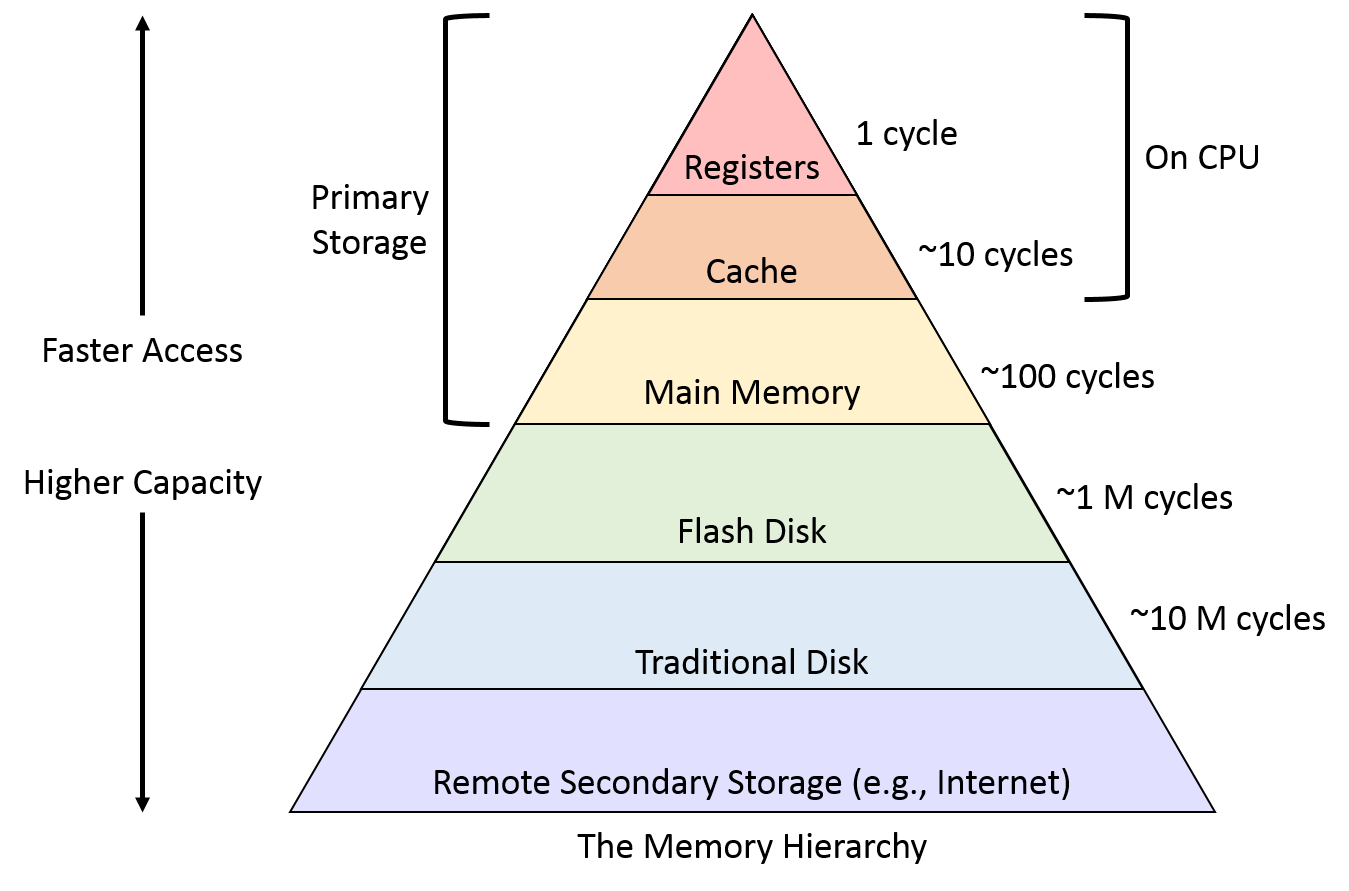
\includegraphics[width=1.0\textwidth]{figures/MemoryHerarchy.png}
    \label{fig:MemoryHerarchy}
  \end{figure}
\end{frame}

\section{Defensive Programmig}

\begin{frame}{Defensive Programmig. Expect the unexpected}
  
Defensive programming is a bit like always wearing a full suit of armor. It’s about preparing for the worst while hoping for the best, much like someone living in a zombie apocalypse with a bunker full of canned goods. In this approach, every function call is a potential trick, every user input a Trojan horse, and paranoia isn’t just recommended, it’s required!

\begin{figure}[h]
  \centering
  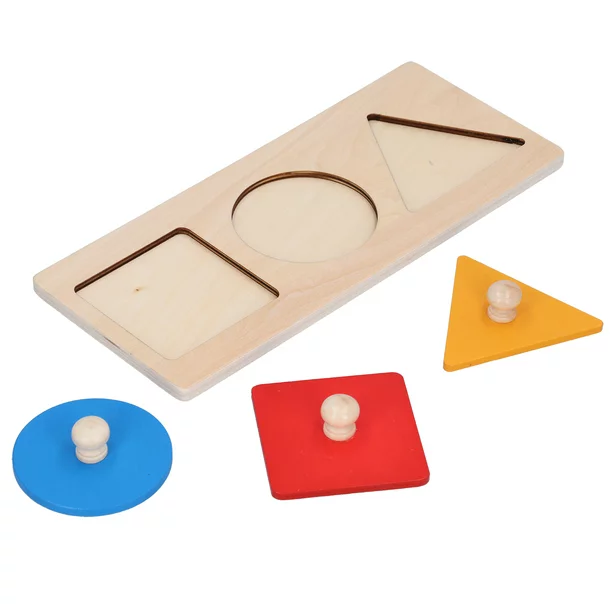
\includegraphics[width=0.25\textwidth]{figures/BadDummpyProof.png}
  \label{fig:BadDummpyProof}
\end{figure}

\begin{figure}[h]
  \centering
  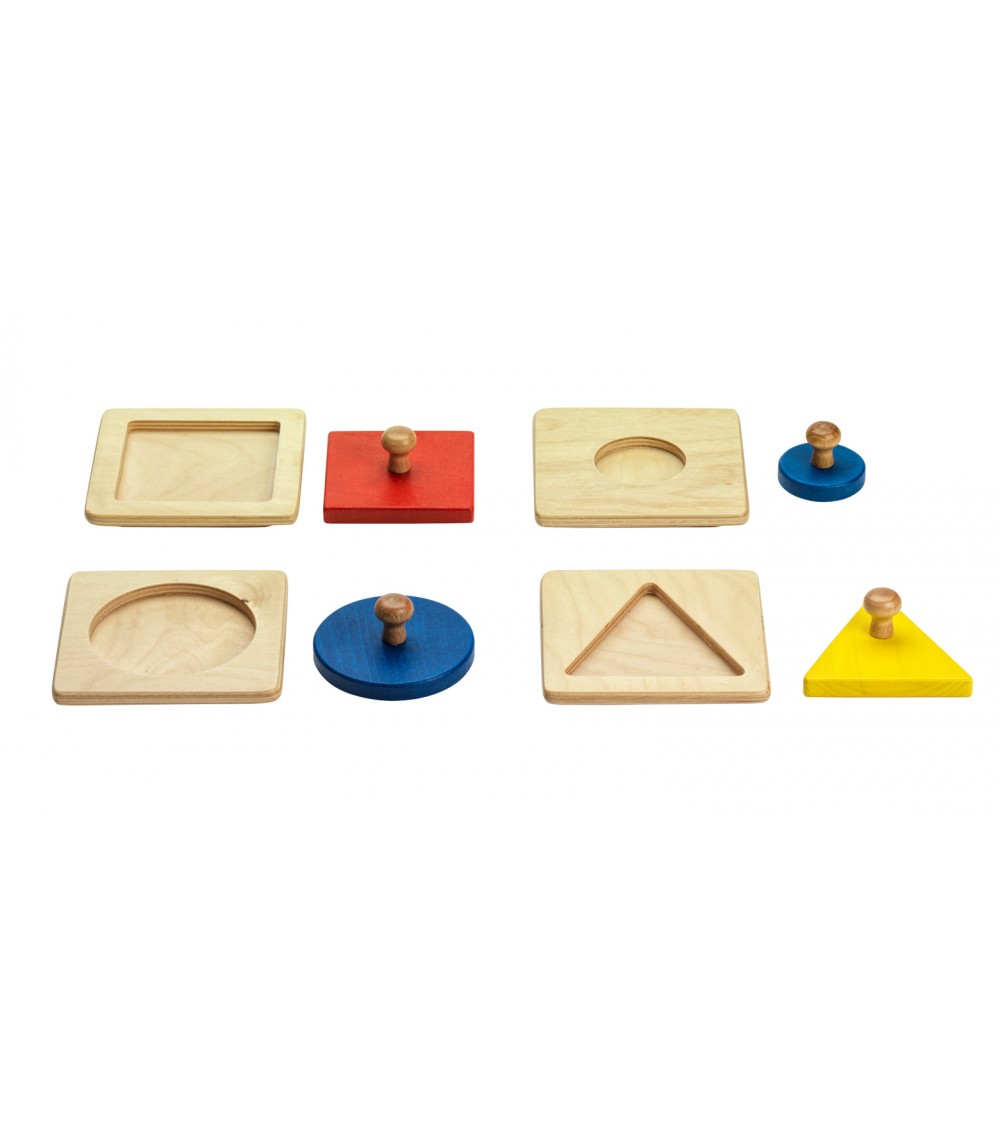
\includegraphics[width=0.5\textwidth]{figures/GoodDummyProof.png}
  \label{fig:BadDummpyProof}
\end{figure}

\end{frame}


\begin{frame}{Common errors in variable allocation}

\end{frame}

\begin{frame}{What does static mean?}

\end{frame}

\begin{frame}{Stack Memory}

\end{frame}

\begin{frame}{Heap Memory}

\end{frame}

\begin{frame}{Pointers}

\end{frame}

\begin{frame}{Callbacks}

\end{frame}

\end{document}